\section{IO testing}
\textbf{Выданные параметры:} [ioport,io-uring]
Система до использования stress-ng:\\
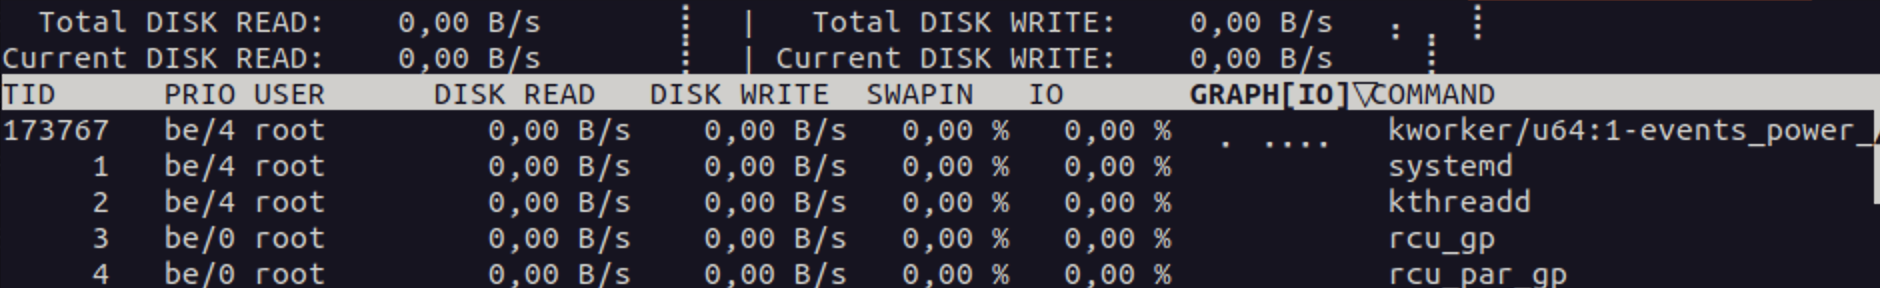
\includegraphics[width=\textwidth]{./io/image/iotop-before.png}
\subsection{ioport}
Из документации stress-ng:
\nquote{--ioport N}{ start  N workers than perform bursts of 16 reads and 16 writes of ioport 0x80 (x86 Linux
systems only).  I/O performed on x86 platforms on port 0x80 will cause delays on the CPU
performing the I/O.}
Сначала найдем оптимальное значение воркеров. Для этого напишем скрипт:
\lstinputlisting[]{io/scripts/ioport-bogops.zsh}
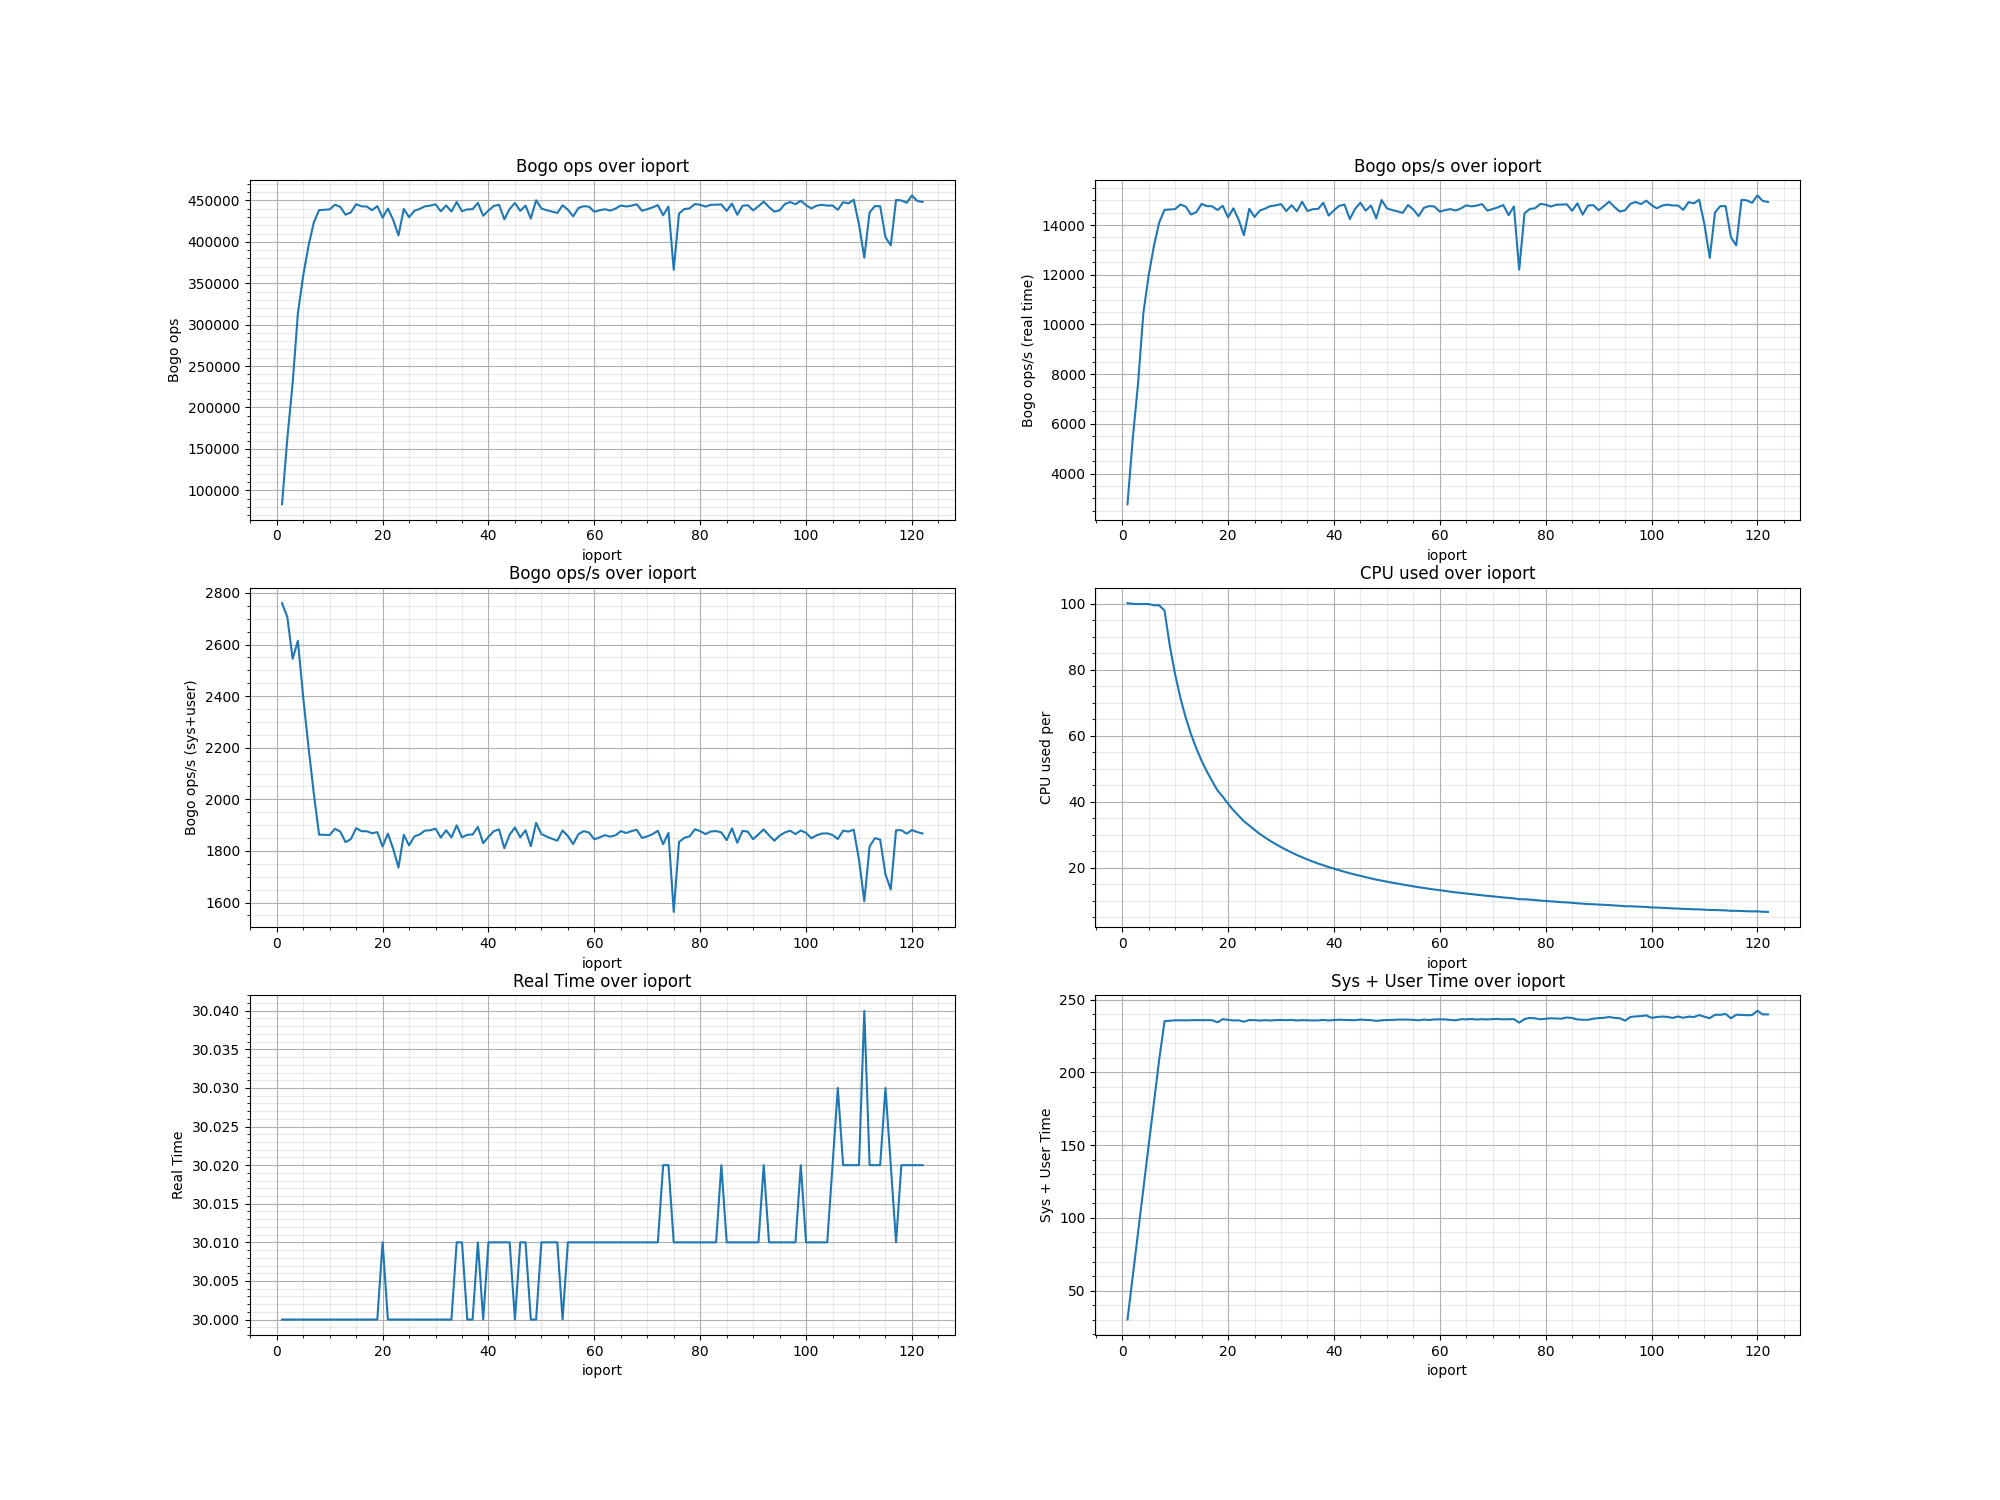
\includegraphics[width=\textwidth]{./io/image/ioport-bogops.png}
Как мы видим, к \textbf{8} воркерам мы достигаем максимального количества bogo ops и далее они не растут.
Проведем анализ нагрузки с помощью \textit{iostat} для этого напишем скрипт:
\lstinputlisting[]{io/scripts/ioport-iostat.zsh}
\nquote{r/s, w/s, d/s, f/s}{запросов на чтение, запись, усечение и синхронизацию, выполняемых дисковым устройством в секунду (после слияния);}
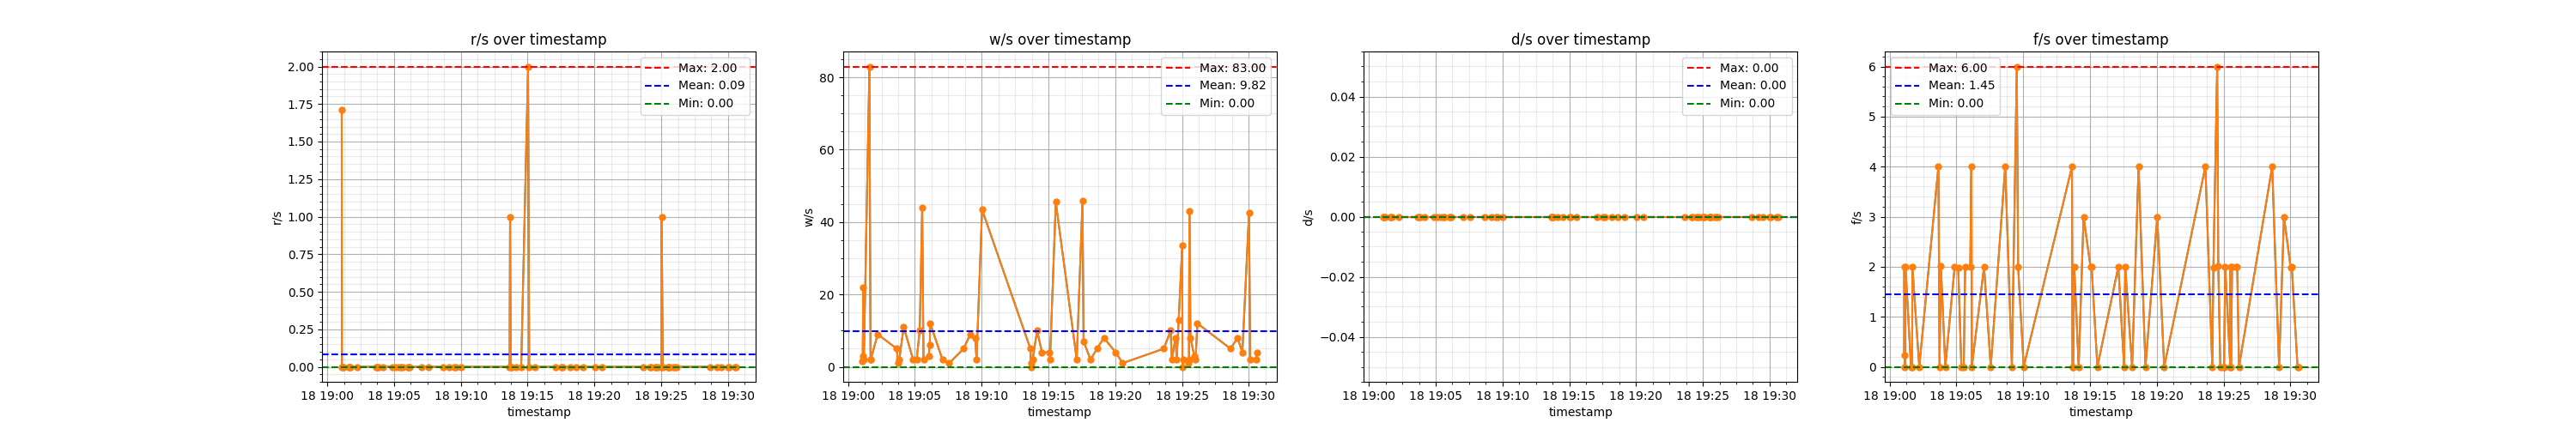
\includegraphics[width=\textwidth]{./io/image/iostat_1.png}
Видим, что запросов на чтение значительно меньше и они реже, чем запросы на запись. Также у нас не было запросов на освобождение блоков на диске (команда ATA TRIM). Мы можем заметить запросы на синхронизацию, которых сильно меньше чем запросов на запись, но они чаще.
\nquote{rkB/s, wkB/s, dkB/s}{объем чтения, записи и усечения в килобайтах в секунду;}
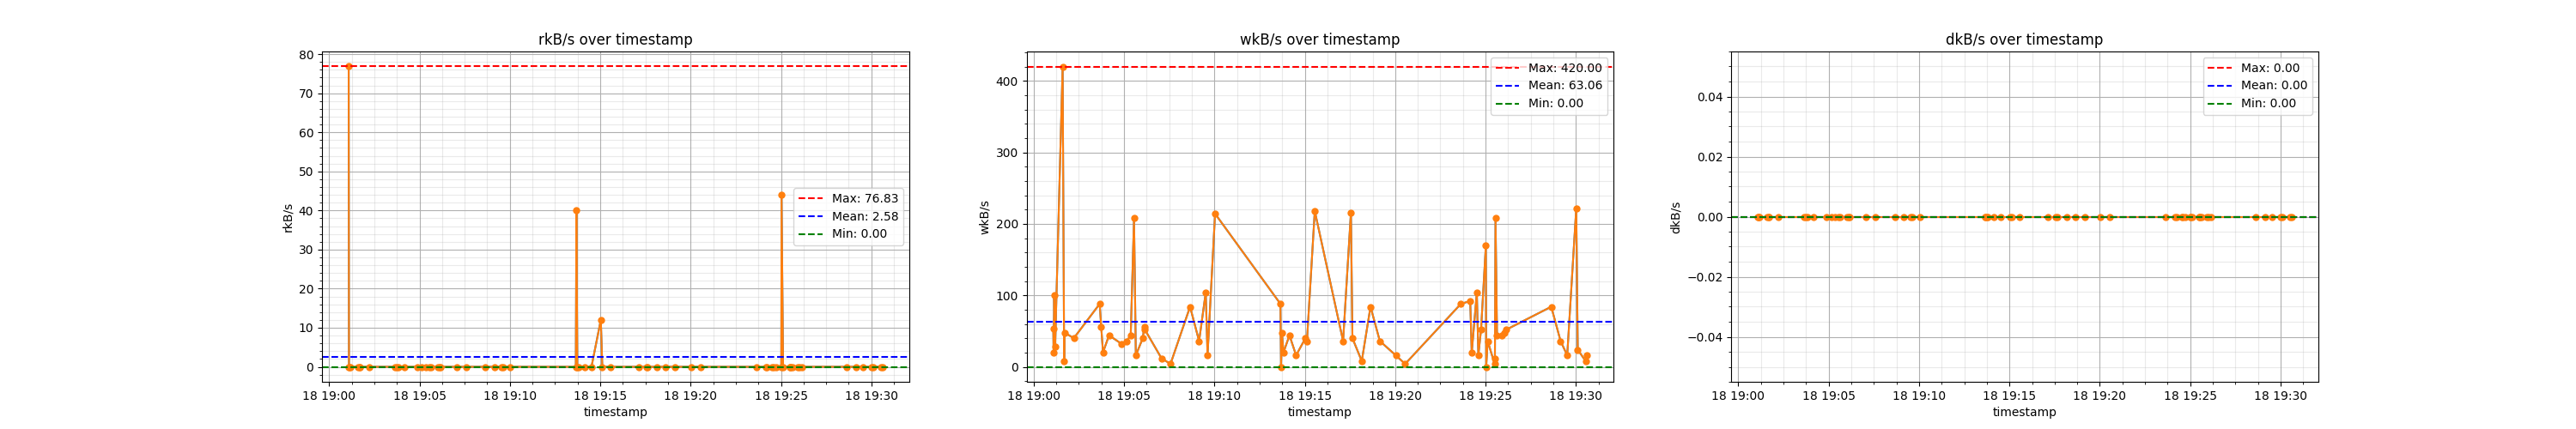
\includegraphics[width=\textwidth]{./io/image/iostat_2.png}
Из графиков видно, что мы читаем меньше, чем записываем. Читали мы максимум чуть меньше 80 Кб/c, записывали максимум чуть больше 400 Кб/c и около 60 Кб/с в среднем.
\nquote{\%rrqm/s, \%wrqm/s, \%drqm/s}{количество запросов в секунду на чтение, запись и усечение, добавленных в очередь и объединенных, в процентах от общего количества запросов каждого типа}
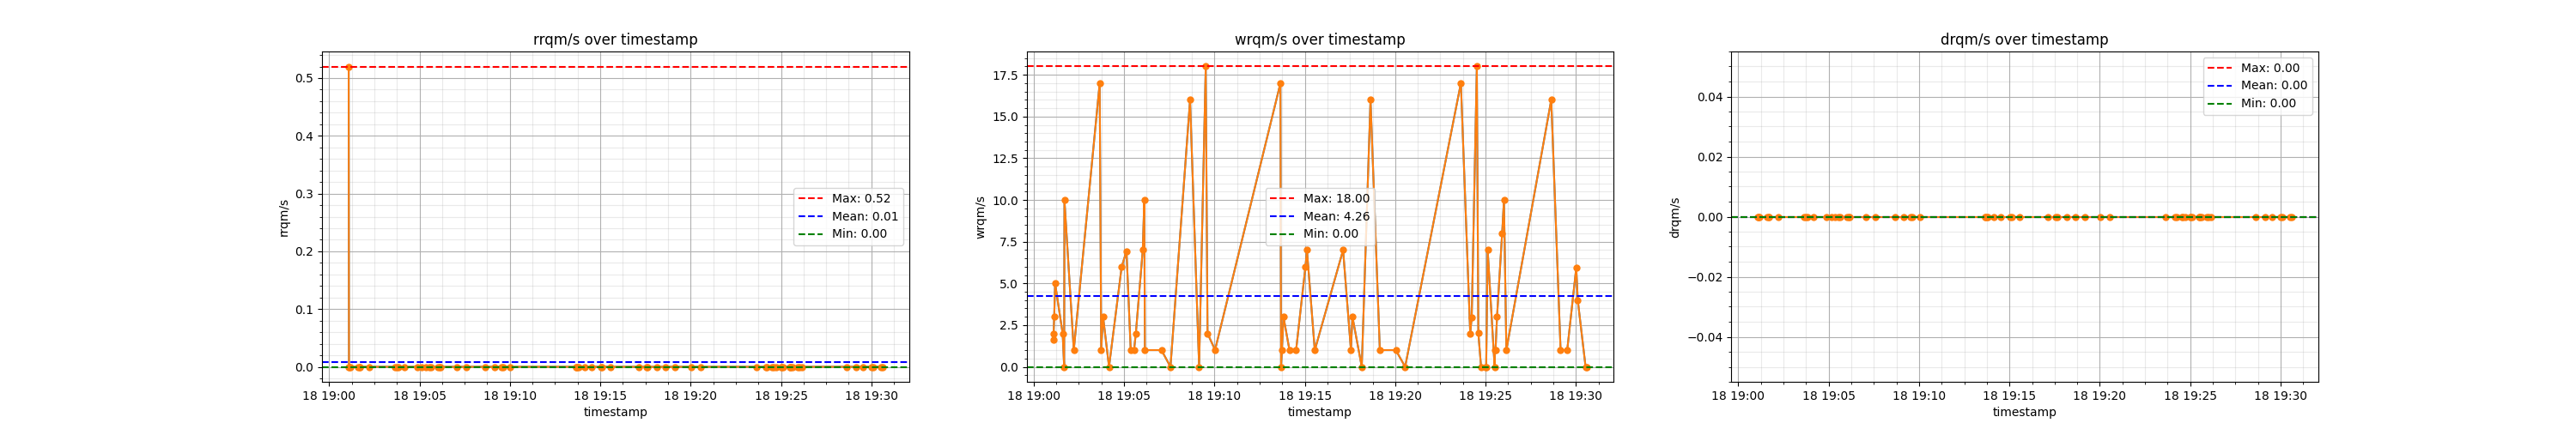
\includegraphics[width=\textwidth]{./io/image/iostat_3.png}
Видим, что запросы на чтения практически не объединялись, в то же время около 4\% запросов из очереди на запись были объединены.
\nquote{\%rrqm, \%wrqm, \%drqm}{количество запросов на чтение, запись и усечение, добавленных в очередь и объединенных, в процентах от общего количества запросов каждого типа}
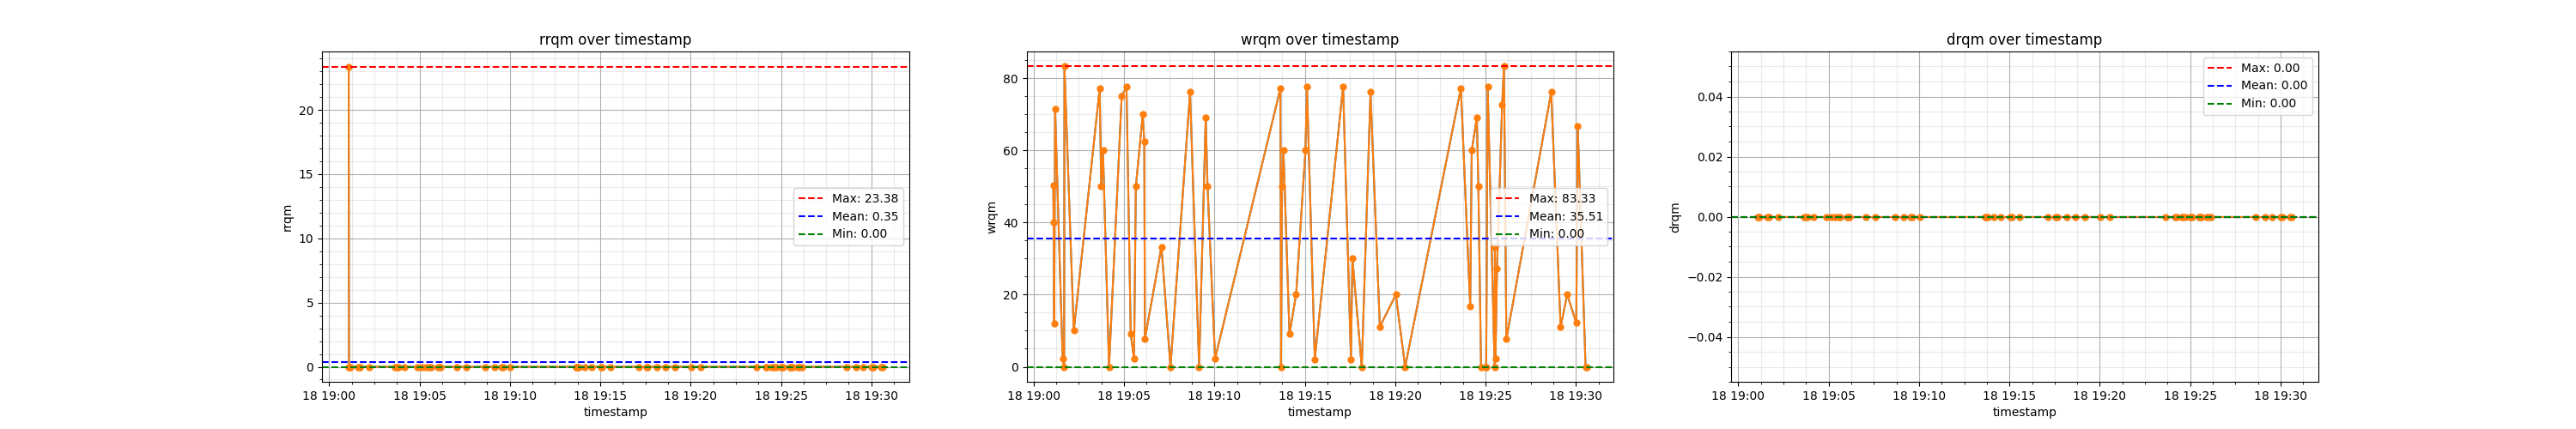
\includegraphics[width=\textwidth]{./io/image/iostat_4.png}
Вывод, тот же что и выше.
\nquote{r\_await, w\_await, d\_await, f\_await:}{среднее время отклика для чтения, записи, усечения и синхронизации, включая время ожидания в очереди драйвера и время отклика устройства (миллисекунд);}
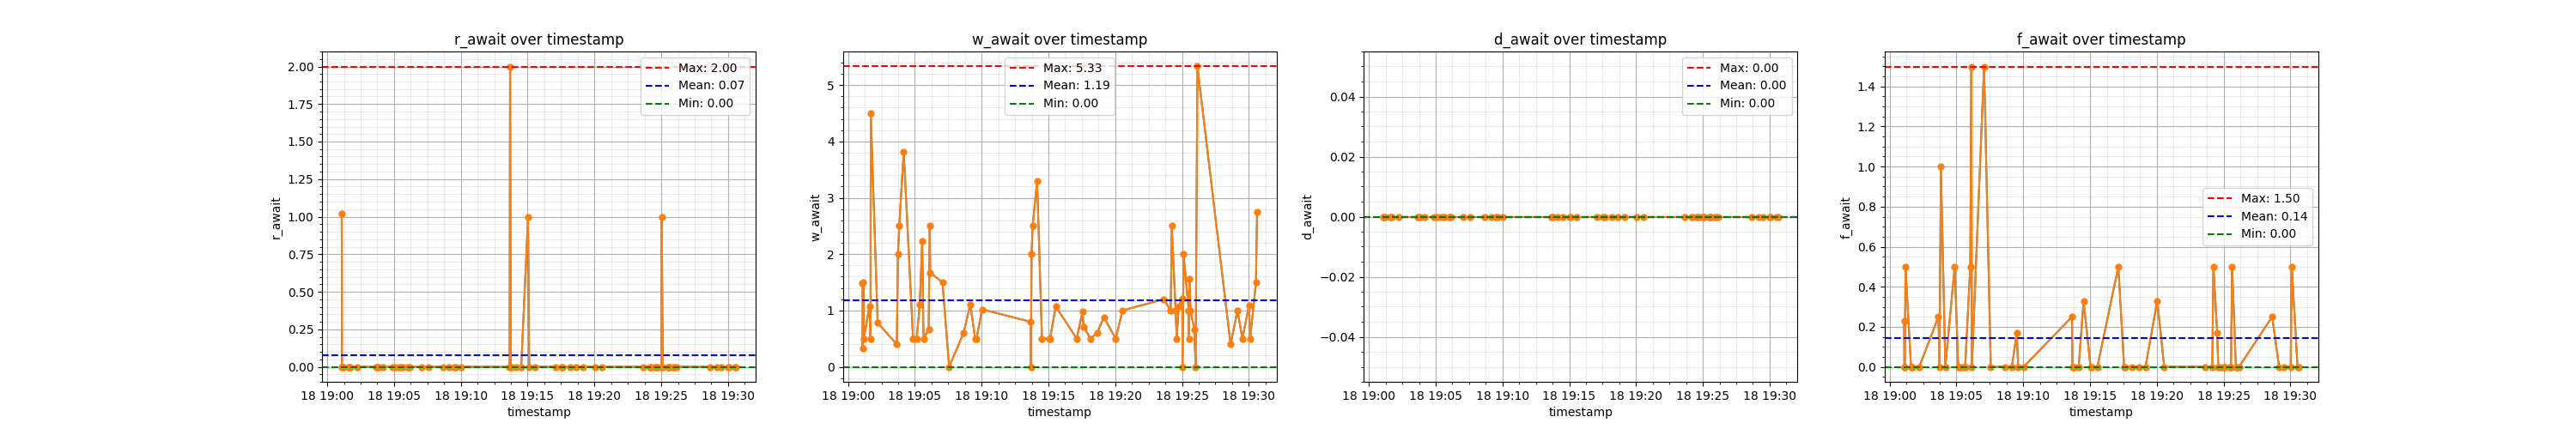
\includegraphics[width=\textwidth]{./io/image/iostat_5.png}
Видим, что время отклика на чтение максимум было 2 миллисекунды (1 раз), 1 миллисекунда (3 раза) и практически моментально все остальное время.\\
Запись максимум было около 5 миллисекунд, в среднем около 1 миллисекунды.  \\
Синхронизация в среднем имела отклик около 0.14 миллисекунд.
\nquote{reduq-sz, wareq-sz, dareq-sz}{средний размер чтения, записи и усечения (килобайт).}
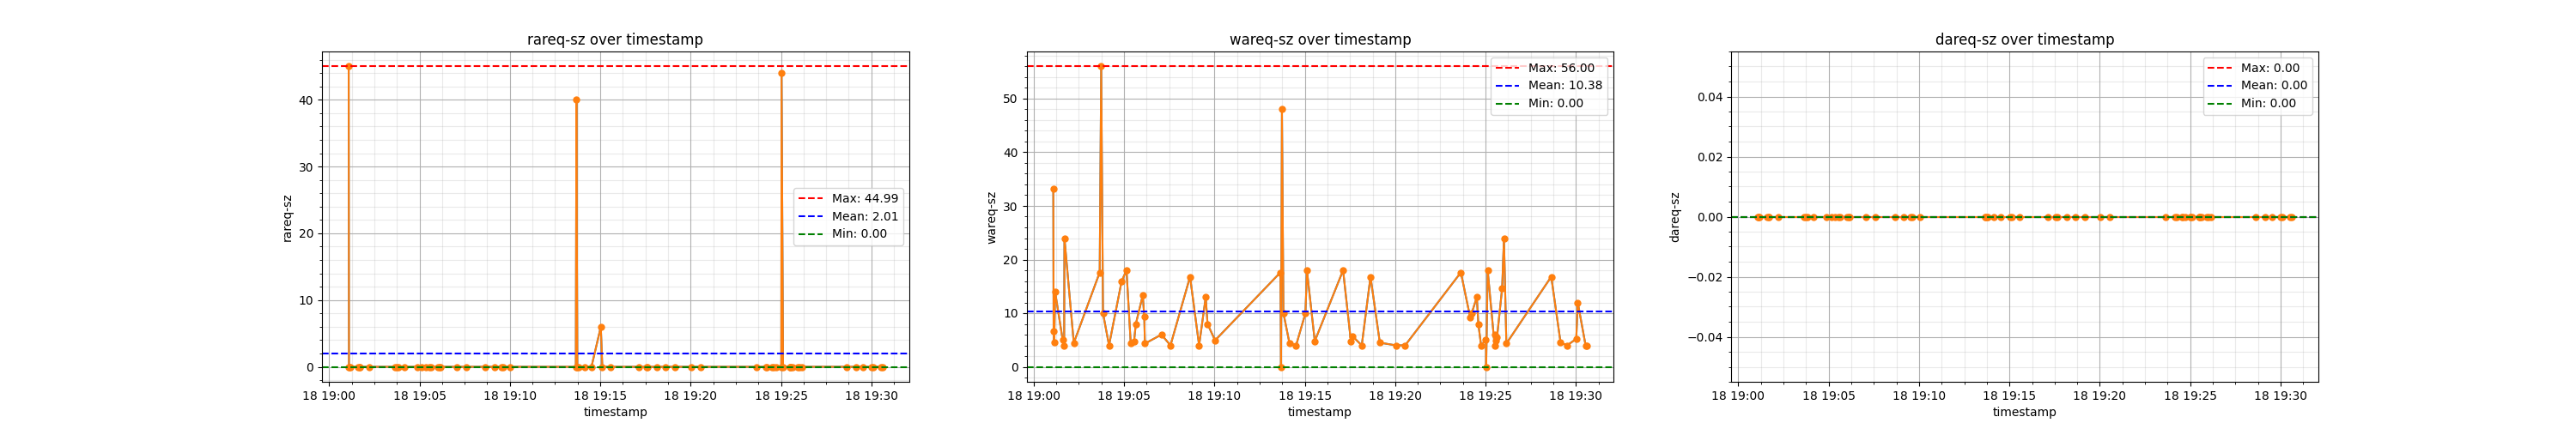
\includegraphics[width=\textwidth]{./io/image/iostat_6.png}
Видим, что мы читали редко и сразу много около 40 килобайт.\\
Записывали мы частно, но по немного (в среднем по 10 килобайт).\\
\nquote{aqu-sz}{cредняя длина очереди запросов, которые были отправлены устройству.}
\nquote{\%util}{процент прошедшего времени, в течение которого устройству были отправлены запросы ввода-вывода (использование полосы пропускания устройства).}
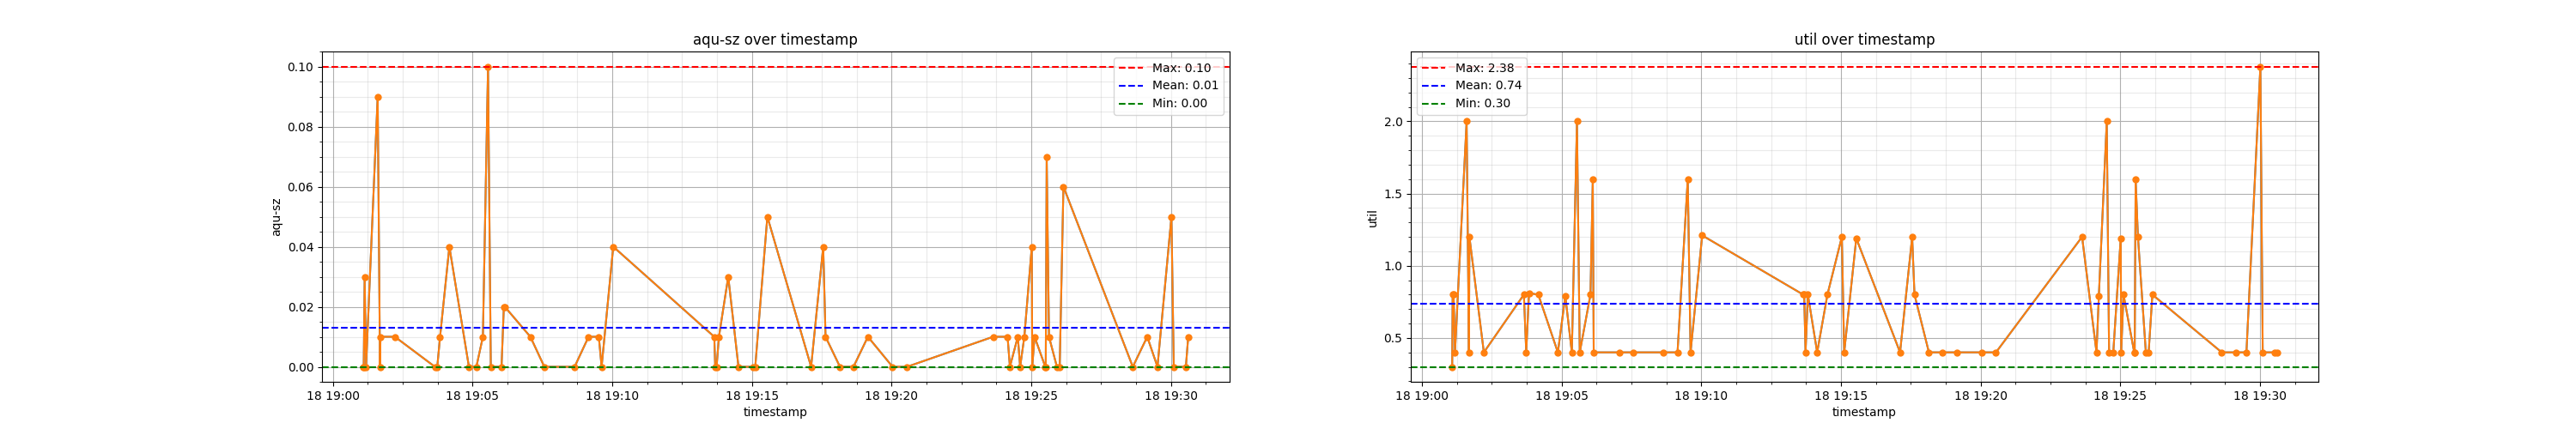
\includegraphics[width=\textwidth]{./io/image/iostat_7.png}
Из графиков видно, что в среднем очередь запросов была небольшой. Также полосо пропускания была большей части свободна.
\textbf{Вывод:} зачем я это  вообще делал? В документации ведь ясно сказано, что мы не нагружаем диск, а только обращаемся к ioport 0x80, тем самым нагружаем только CPU.
И все это чтение и запись это шум от других программ.
\nquote{--io-uring N}{start  N workers that perform iovec write and read I/O operations using the Linux io-uring interface. On each bogo-loop $1024
\times 512$ byte writes and $1024 \times$ reads are performed on a temporary file.}
